
\chapter{ Movimento de um corpo em queda vertical: determinação da aceleração da queda}
\label{chap:acelera}


\vspace{-0.7cm}

\section{Introdução}
Neste experimento determinaremos a aceleração de um corpo em queda vertical e vamos 
comparar o resultado obtido com o valor de referência da aceleração da gravidade ($g$)
para a cidade de Rio de Janeiro. 

Vamos analisar o movimento de queda vertical de um corpo cuja forma e tamanho apresente uma força de resistência do ar desprezível (por exemplo uma bolinha de gude) \footnote{Lembre que a queda vertical de um corpo quando a única força atuante sobre ele é a força da gravidade chama-se queda livre.}. Que tipo de movimento 
apresentaria o corpo se a força de resistência do ar fosse desprezível? \footnote{Lembre que o movimento da partícula é determinado através da Segunda Lei de Newton.}

Pense sobre o planejamento desse experimento. A aceleração do corpo pode ser obtida diretamente? Quais grandezas devem ser medidas para que seja possível obtê-la? Quais instrumentos são mais adequados para que esses dados possam ser coletados?

O experimento será discutido e guiado pelo roteiro abaixo. Siga o roteiro e as orientações do professor 
nos encontros remotos e vá fazendo suas anotações no caderno de laboratório. 

\section{Procedimento Experimental}

O arranjo experimental experimental está mostrado na Figura~\ref{fig:experimento}. Escolha uma bola de gude ou qualquer corpo arredondado de dimensões da ordem de grandeza da bolinha mostrada na Figura~\ref{fig:experimento}. Você deverá filmar a queda da bolinha com um celular, desde uma altura de, mais o menos, um metro. Para isso peça ajuda a uma pessoa que vai segurar a bolinha enquanto você filma.  Cole na parede uma régua de papel como está indicado na Figura~\ref{fig:experimento} \footnote {A régua não precisa ter a extensão de toda a trajetória a ser filmada, é somente uma referência de escala.}. Para a filmagem, posicione o celular num apoio com a tela do celular paralela à parede onde está colada a régua de papel. O celular deverá estar posicionado mais o menos no meio da trajetória da bolinha a uma distância da parede suficiente para poder filmar toda a queda de mais ou menos um metro. Não use ``slow-motion'' (câmera lenta),  filme com a velocidade normal do seu celular. A imensa maioria dos celulares filma a uma taxa de 30 frames/s \footnote{A palavra em inglês ``frame'' significa quadro.}. Verifique no seu celular se essa é a taxa usada.

Para analisar o filme da queda será usado o aplicativo Tracker para uso num computador 
que poderá ser baixado gratuitamente no link: 
\href{https://physlets.org/tracker/}{\textcolor {blue}
{https://physlets.org/tracker/}}
\footnote {O aplicativo é disponibilizado para os sistemas operacionais Windows, Linux e Mac OSX.}. 
O filme também poderá ser analisado com o aplicativo VidAnalysis disponível gratuitamente para celulares com sistema operacional Android no link  do
\href{https://play.google.com/store/apps/details?id=com.vidanalysis.free}{\textcolor {blue}
{Google Play}}. 
Os tutoriais de uso destes aplicativos estão disponíveis na forma de vídeos no site da \href{https://fisexp1.if.ufrj.br}{\textcolor {blue} {Física Experimental 1}} . 
No final do roteiro, encontram-se o Apêndice~\ref{sec:tracker} um tutorial básico do aplicativo Tracker, e um tutorial básico do aplicativo VidAnalysis no Apêndice~\ref{sec:vidanalysis}.  


\section{Análise de dados}
Usando o aplicativo Tracker ou alternativamente o aplicativo  VidAnalysis, monte a Tabela \ref{tabela1}.
\begin{table}[h]
\centering
\begin{tabular}{c|c|c|c|c}
t (s) & $y$ (cm) & $\delta y$ (cm)& $v_y$ (cm/s)& $\delta v_y$ (cm/s)\\
\hline 
&&&&  
\end{tabular}
\caption{Tabela de dados da experiência.}
\label{tabela1}
\end{table}
As colunas do tempo $t$ e da posição $y$ são preenchidas usando os aplicativos Tracker ou  VidAnalysis. As coordenadas $y$ correspondem às posições, por exemplo, do centro da bolinha ao longo da trajetória de queda, após ter escolhido o sistema de referência. Note que ao longo da trajetória a imagem da bolinha pode ficar um pouco embaçada como na Figura~\ref{fig:reguacomxis}.
Nesse caso, foi marcado com um ``x''  em azul 
o centro da bolinha enquanto que a barra vermelha é uma escolha razoável da região de incerteza
da posição do centro da bolinha.  

Para preencher a coluna da velocidade $v_y$ leia o Capítulo~\ref{sec:vinst} da Apostila.
Como são calculadas as incertezas $\delta v_y$?
\begin{itemize}
\item Em um papel milimetrado desenhe o gráfico $v_y \times t$ a partir dos dados da tabela indicando 
a incerteza nos valores das velocidades. Qual é a forma esperada para este gráfico?
\end{itemize}

  \begin{minipage}{\linewidth}
      \centering
      \begin{minipage}{0.25\linewidth}
          \begin{figure}[H]
              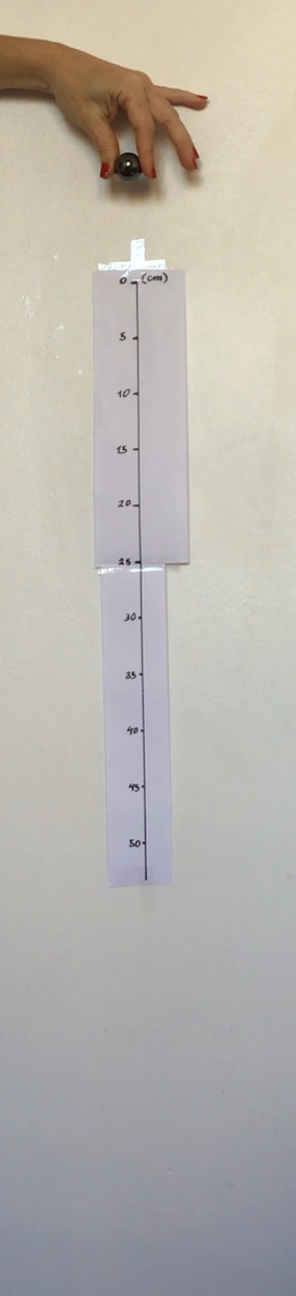
\includegraphics[width=\linewidth]{Figuras_exp3/fig1.pdf}
              \caption{\label{fig:experimento} Dispositivo experimental. Não esqueça de colar na parede uma régua de papel, como a indicada na Figura, para ser usada como referência na análise de dados.}
          \end{figure}
      \end{minipage}
      \hspace{0.05\linewidth}
      \begin{minipage}{0.3\linewidth}
          \begin{figure}[H]
              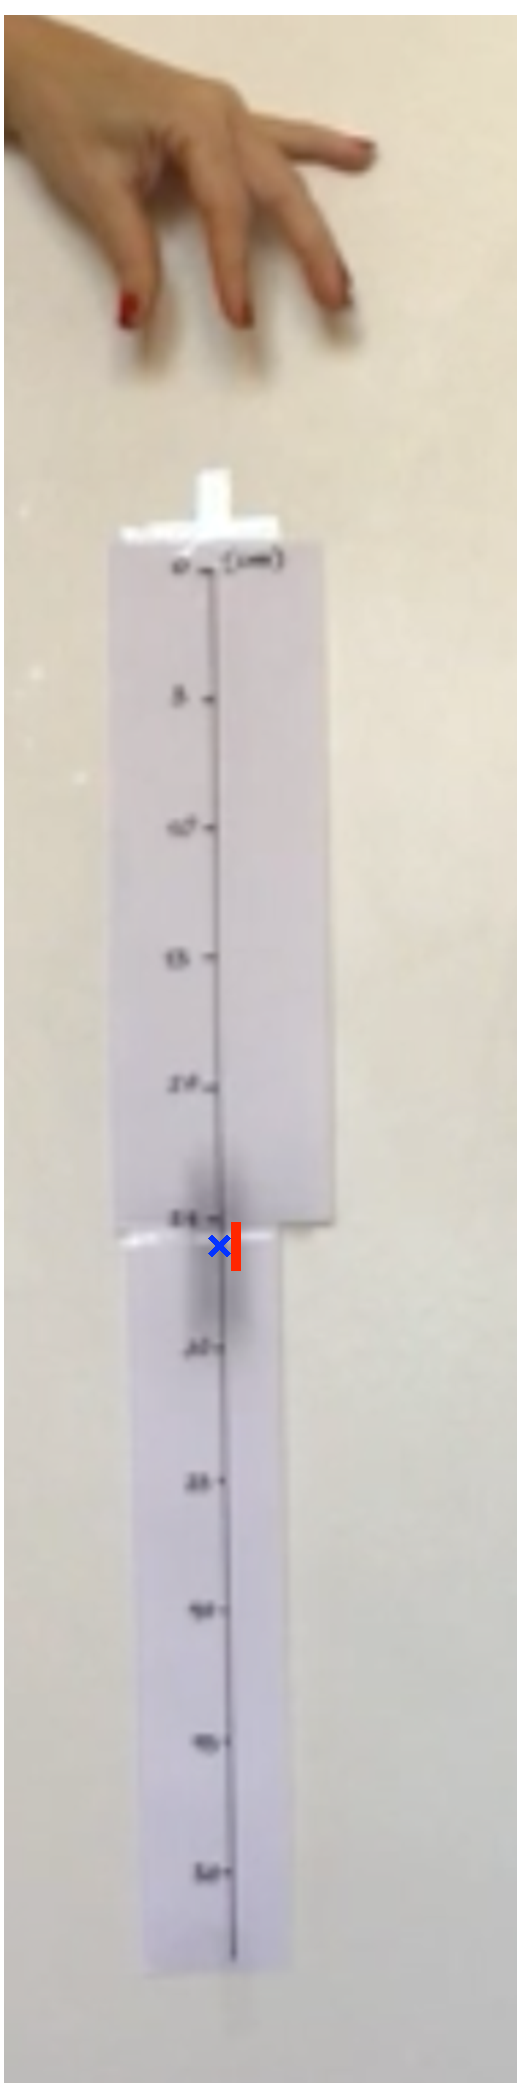
\includegraphics[width=\linewidth]{Figuras_exp3/fig2roteiro.pdf}
              \caption{\label{fig:reguacomxis}  Imagem da bolinha em plena queda. Note-se que a imagem, devido à alta velocidade, fica um pouco embaçada.}
          \end{figure}
      \end{minipage}
  \end{minipage}%

\begin{itemize}  
\item Use as colunas $t$, $v_y$ e $\delta v_y$ para  calcular através do Método dos Mínimos Quadrados (Seção~\ref{chap:minquad}  do Capítulo Conceitos Básicos para Análise de Dados da Apostila), qual é a melhor reta que aproxima os dados experimentais do gráfico $v_y \times t$?
\item Com os parâmetros da reta obtida no item anterior,  desenhe-a  na mesma folha de papel milimetrado 
onde fez o gráfico $v_y \times t$. Se você não conseguir achar um aplicativo que implemente o ajuste linear pelo método dos mínimos quadrados, desenhe a melhor reta que aproxima os dados experimentais 
pelo método visual (ver Seção~\ref{chap:minquad} do Capítulo Conceitos Básicos para Análise de Dados da Apostila) e obtenha os parâmetros que definem a reta 
(coeficiente angular $a$ e coeficiente linear $b$) escolhendo dois pontos na reta e substituindo na equação da reta $y=a\;t+b$.
\end{itemize}

\section{Discussão dos resultados}
\begin{enumerate}
\item A partir dos parâmetros do ajuste linear aos dados experimentais $v_y$ vs. $t$, 
como se obtêm o valor da aceleração de queda da bolinha?
\item 
Compare o valor da aceleração de queda da bolinha com o valor da aceleração da gravidade 
para a cidade do Rio de Janeiro que é $g=(978,7\pm 0,1)$ cm/$s^2$). 
Qual valor é mais preciso? Você utilizaria este método para determinar o valor da gravidade? Justifique.
\end{enumerate}


\section{Opcional: Estudo da conservação da energia}

%Também poderá entregar no arquivo pdf do relatório as seguintes tarefas opcionais:
\begin{enumerate}
\item Utilizando os dados registrados para a posição $y$ como função do tempo $t$, determine a altura $h$ da bolinha para cada instante de tempo, a partir do ponto mais baixo na Tabela~\ref{tabela1}.
\item Determine a energia cinética ($K$), energia potencial ($U$) e a energia mecânica ($E$) para cada intervalo de tempo. Para facilitar a organização das informações, construa uma tabela.
\item Faça um gráfico que contenha a energia cinética, potencial e mecânica em função do tempo.
\item Discuta a partir do gráfico obtido, se há ou não conservação da energia mecânica. Justificar.
\item No caso da energia não se conservar, determine o ganho ou perda percentual.
\end{enumerate}
\underline{\bf Observações:}
\begin{itemize}
\item Para os cálculos de energia considere a aceleração da gravidade no Rio de Janeiro, com 
sendo $g=(978,7 \pm 0,1)$ cm/$s^2$.
%\item Não esqueça de colocar todos os cálculos de propagação de incerteza num Apêndice.
\end{itemize}
\clearpage

\thispagestyle{plain}